%
% File: chap02.tex
%
\let\textcircled=\pgftextcircled
\chapter{Case study}
\label{chap:case_study}

\initial{T}he case study that will be considered for this project is a new SFR technological demonstration reactor design, the \gls{astrid}. Studying such a huge complex system as a nuclear reactor can be daunting and unfeasible in a limited amount of time. In the context of this project, the systems and components that will be studied, as well as the level of details that will be considered, are described in this chapter.


\section{\gls{astrid}}
\label{sec2:astrid}

The ASTRID prototype, a Sodium-cooled pool-type Fast Reactor design, is currently designed by the CEA in Cadarache, France. This research reactor will have a thermal output of 1500 MWth, generating around 600 MWe. The goal of this prototype is to show the improvement in the sodium-cooled fast reactors design area since Superphenix, and most notably demonstrate the minor actinides transmutation possibilities offered by this design.


% A single figure
\begin{figure}[t!]
	\centering
	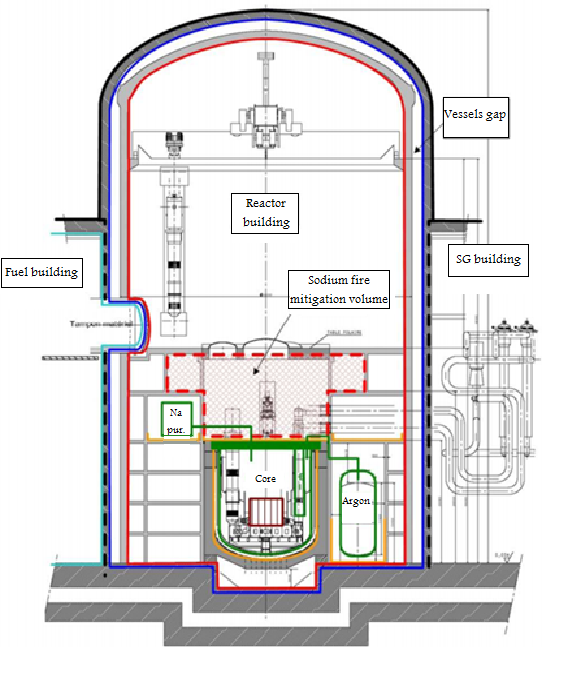
\includegraphics[height=0.75\textheight]{fig02/astrid_simplified}
	\mycaption[ASTRID reactor building generic schematics]{ASTRID reactor building generic schematics}
	\label{fig:c2f1}
\end{figure}

As it represents the future of this reactor design option in France, and, if successful, potentially a larger scope internationally, this reactor will act as the case study. In that regards, this document aims to show how well the design respond to recent engineering methods for risk and reliability analysis, in the event of significant incidents and loss of functionality, and to discuss how the findings can be accurately passed onto the public opinion. Moreover, it will consider the reliability aspect during some transient situation, in order to identify and mitigate the loss of electrical power generation.


%=======
\section{Case study}
\label{sec2:case_study}

During this case study, state-of-the-art risk and reliability analysis methods will be applied to the system. The main failures of interest will be put in two categories, risk and reliability. The risk, or safety, failures are those that can cause a core meltdown or a radioactive contamination of the environment or workforce, either by themselves or combined with one or more uncoupled failures. The reliability failures are the ones that would cause a loss of electricity generation, and thus render the whole system mostly inoperant. It is interesting to consider the fact that for this particular system, the loss of electricity generation capability is not by itself sufficient to deem the system inoperable, since the secondary plant objective, minor actinides transmutation, could still be taking place. Thus, by intended system goals, reliability issues are mitigated due to their diversity.

The system of interest is defined as including the components identified within the following sections. Due to scarce publicly available information on the detailed reactor designed, notably redundancies, the author has exerted his judgement and experience as a nuclear engineer to use a model deemed representative of reality.

\subsection{Generic}
\label{subsec2:generic}

This category contains components which are found throughout the plant and are identified as a cause of likely failures, according to historical data. For example, pipes and valves can be found in this sections. Depending on the level of details, bolts, screws, and other small component could also be identified.


\subsection{Reactor core}
\label{subsec2:core}

This reactor core design presents several natural objectives:
\begin{itemize}  
\item No sodium boiling 
\item Negative sodium void effect 
\item No fuel pellet meltdown
\item High performance (cycle length and fuel burn-up)
\end{itemize}

\newacronym{cfv}{CFV}{Coeur a Faible Vidange, Low Void Worth Core}

Those objectives should be met by design. Consequently, a type of core (\gls{cfv},~\cite{mschenaud01}), optimized for low sodium void effect, has been developed by the CEA. This does not mean that such risk or reliability failures will now be ignored, but they will be classified as less likely to occur.

The main components of the reactor core that will be considered are:
\begin{itemize}
\item Fuel assemblies

    The fuel assemblies contains the radioactive fuel elements

\item Control rods 

    The control rods allows the emergency shutdown of the chain reaction and the modulation of the power output.

\item Neutron detectors

    These detectors gives precious information on the neutron activity inside the core.

\item Thermocouples

    These temperature detectors give needed information on the temperature within the fuel and in the primary sodium.
\end{itemize}


\subsection{Reactor structure}
\label{subsec2:structure}

This category includes the different vessels and concrete elements in the whole system. Two main types can be identified, the structure surrounding the primary circuit and the ones surrounding the secondary circuit and other. For the primary circuit, those are notably:
\begin{itemize}
\item Inner vessel

    This structure separates the hot primary sodium from the cold primary sodium.

\item Main vessel 

    This is the main vessel, separating the primary circuit from the secondary circuit and the environment.

\item Safety vessel

    This is an envelope of the main vessel insuring supplementary containment.

\item Roof

    This can be considered part of the main vessel, but it does support other components, and as such is treated differently.

\item Core catcher

    This is a safety system in case of a meltdown, to prevent the corium from spilling out of a controlled area.
\end{itemize}

For the secondary circuit and other systems, those can be:

\begin{itemize}
\item Command room

    This structure houses the command controls.

\item Intervention paths

    This includes the tunnels or hallways leading to different parts of the site.

\item Secondary systems building

    This building houses the turbines, condensers, secondary electromagnetic pumps, and other secondary systems and elements.

\item Spent fuel pools

    This element allows for stocking the spent and new fuel assemblies before, during or after a fuel loading.
\end{itemize}

In this case study, only the primary systems structure will be considered. However, secondary structures failures might also be identified in some failure modes.

\subsection{Primary circuit components}
\label{subsec2:primary}

The considered components in the primary circuit are:

\begin{itemize}
\item Reactor Core

    This component was introduced in greater details in~\ref{subsec2:core}. It could be separated from the primary circuit depending on the depth of the analysis.
    
\item Intermediate heat exchanger (redundancy: 4)

    This component transfers heat from the sodium in the primary circuit to the sodium in the secondary circuit.

\item Primary mechanical pump (redundancy: 3)

    This component allows for circulating the primary sodium through the core.

\item Decay heat removal components (redundancy: 2)

    These components and systems insure the safety function associated with cooling the core.

\item Argon tank

    This element permits to keep the sodium away from oxygen, with which it can react.

\item Sodium purifier

    This component purifies the primary sodium to clean it from foreign elements and chemicals
\end{itemize}


\subsection{Secondary circuit components}
\label{subsec2:secondary}

The considered components in the secondary circuit are:

\begin{itemize}
\item Secondary electromagnetic pump (redundancy: 4)
\item Steam generator (redundancy: 4)
\end{itemize}


\subsection{Tertiary circuit components}
\label{subsec2:tertiary}

The considered components in the tertiary circuits are:

\begin{itemize}
\item Turbine (redundancy: 3)
\item Generator (redundancy: 2)
\item Condenser (redundancy: 3)
\item Heat sink
\end{itemize}
